\chapter{Blockchain as the Infrastructure of Semantic Web}
In more and more places throughout the world, transactions involving numerous parties are represented by distributed ledgers. Without an index, it is challenging to search for specific data in a distributed ledger. As a result, indexing data in the distributed ledger is a prerequisite that gives users the capacity to search across many ledgers, hence boosting the system's functionality and usability \cite{Third}.
\section{Distributed Ledgers and Indexing}
A distributed ledger built on a blockchain lacks centralized management. Multiple blocks make up a blockchain; the first block is manually made, and subsequent blocks are added by some sort of consensus mechanism amongst nodes. \\
With the help of an Ethereum smart contract, it is possible to autonomously handle transactions on the blockchain without involving any dubious third parties. The accounts used by Ethereum smart contracts often have the ability to store data, change it, or carry out operations using input and output.
Data must be indexed since smart contracts are time-ordered and hold information in blocks. By indexing the smart contract, we are able to explore, evaluate, and utilize the distributed ledger's services, as well as expose them to the outside world for more interactions. \\
There are various indexing levels for smart contracts: The fundamental level for the following step is the basic level. Data can be stored or accessed here, and it indexes fundamental distributed ledger entities like accounts and blocks. Smart contracts have many functional interfaces that represent the additional capabilities of systems like Ethereum at the functional level \cite{Third}.
\subsection{Why Do We Use Ontology for Blockchain?}
Blockchain often uses a cloud computing architecture and is a distributed database that is copied across all nodes. In other words, the database contains data that is dispersed among numerous organizations. In order for data to be properly understood by organizations, there needs to be a standard interpretation. These interpretations are applicable through a formal specification that allows for verification and inference in network-based software and applications. \\
Here, ontology is crucial in ensuring that various enterprises have a common interpretation of the data in the shared database.\\
Blockchain as a modeling form uses a different type of ontology \cite{Kim}: \\
\\
\textbf{\textit{Informal/Semi-Ontology}} facilitates search and enhances a better understanding of the business process for developing and applying on the blockchain \cite{Kim}. \\
\\
\textbf{\textit{Formal Ontology}} helps  the formal specification in automating inference and validating the blockchain's functionality. In other words, formal ontology-based blockchain can help in the creation of smart contracts that run on the blockchain \cite{Kim}. \\
Ontologies can also be used to store data in the blockchain: On the one hand, it helps people grasp blockchain concepts better. On the other hand, it allows for the interlinking with other linked data to convey formal reasoning and inferences, \cite{Kim}. \\
By describing the transaction in the context of connected data and enabling the graphical representation of the location of such transactions, vocabulary employed inside an ontology increases the transparency of transactions. Consequently, it also improves users' analytical capacity \cite{Kim}.
\begin{center}
	
	
	\begin{figure}[htb!]
		
		\begin{minipage}{0.55\linewidth}
			\centering
			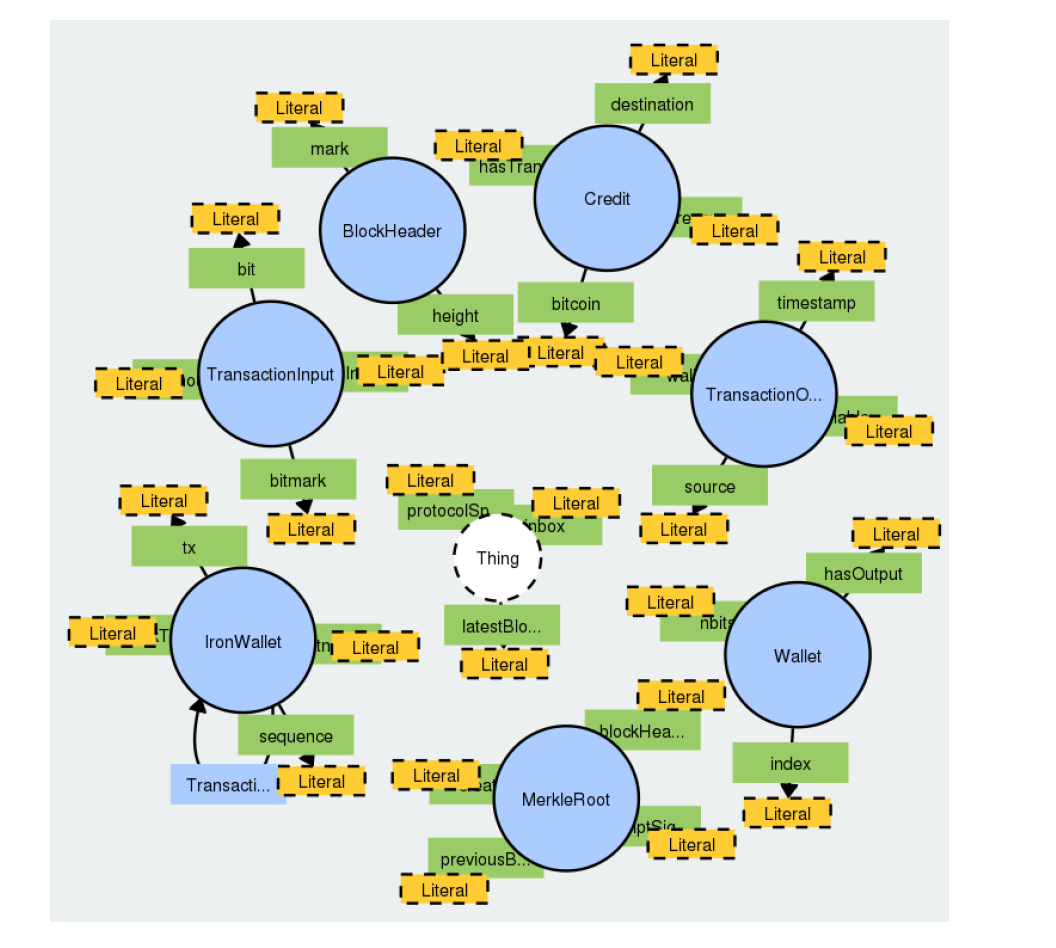
\includegraphics[width=1.65\textwidth]{images/chap02_diagram_ontology.png}
		\end{minipage}
		\caption[Illustration of ontology diagram]{Illustration of ontology diagram \cite{Matthew}}
		
		
	\end{figure}
	
\end{center}
\subsection{Linked Data}
According to Tim Berners-Lee et al., "linked data" is the creation of typed linkages between data from various sources using the Web \cite{Tim}. When information is presented as linked data, it is easy to obtain relevant additional information and link new information to it.
\textit{Berners-Lee} described four rules for linked data:\\
\textbf{- URIs} (Uniform Resource Identifier) as names.\\
\textbf{- HTTP} to search for names.\\
\textbf{- SPARQL, RDF} provide related information about what a user is looking for. \\
\textbf{- Link} to other URLs to provide more information \cite{Hector}.\\

\begin{center}
	\begin{figure}[htb!]
		
		\begin{minipage}{0.55\linewidth}
			\centering
			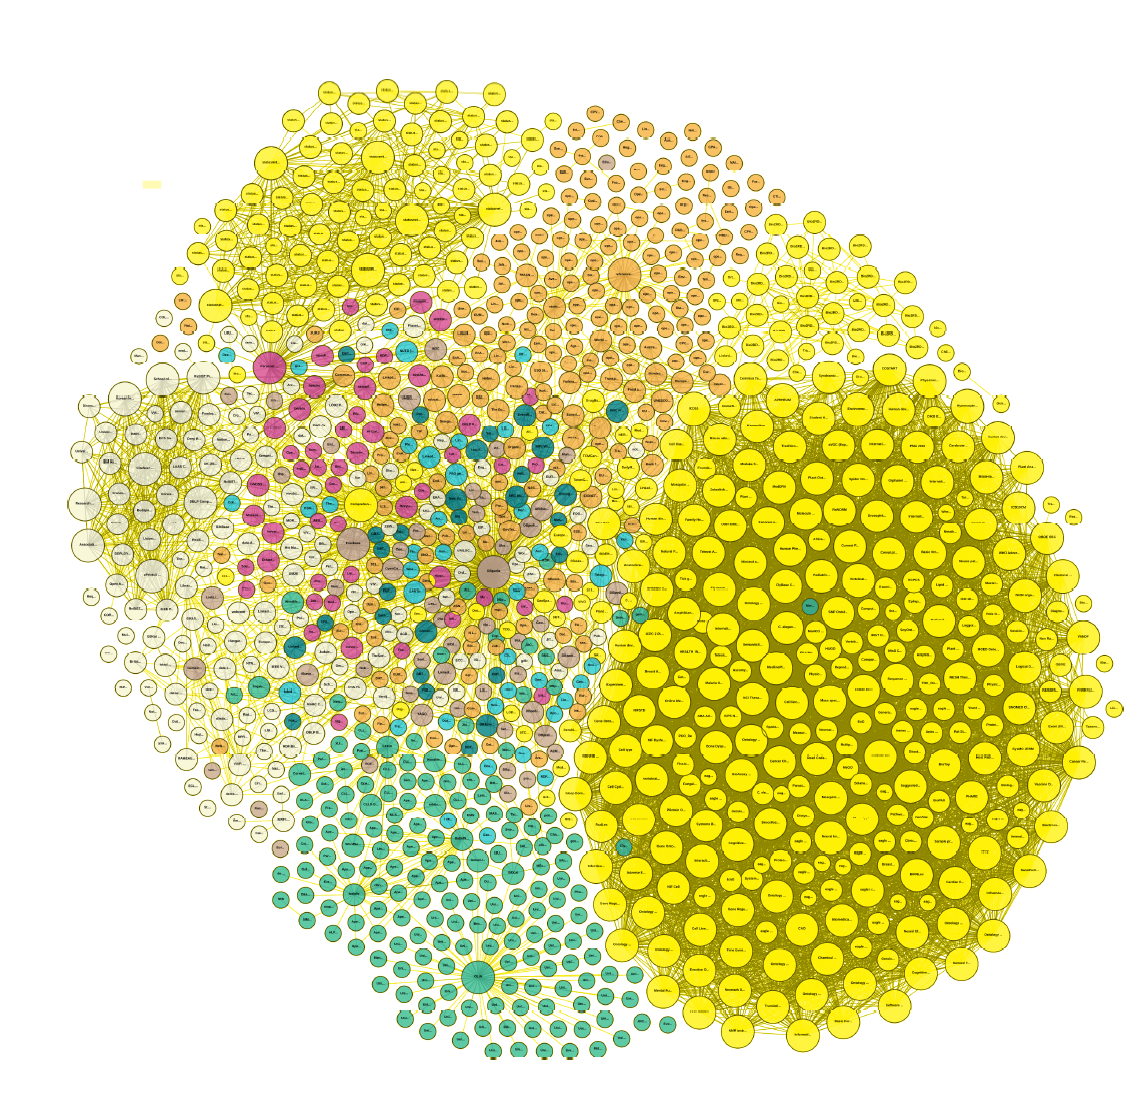
\includegraphics[width=1.55\textwidth]{images/chap02_LinkData.png}
		\end{minipage}
		\caption[Linked data diagram]{Linked data diagram \cite{Hector}}
		
		
	\end{figure}
	
\end{center}
\subsection{RDF}
A group of W3C specifications is known as the Resource Description Framework (RDF). Information is described and modeled using RDF. It is referred to as a triple and describes a topic that predicts an object.
i) The topics described by RDF expressions.
ii) Mention certain characteristics, traits, or connections when describing a resource.
The object's name refers to a property or set of values. \cite{Hector}.
\subsection{SPARQL}
It is a semantic query language for a dataset that enables us to retrieve and alter data stored in RDF format known as triples, according to Wikipedia's definition. One, two, or all of a triple's elements can be queried using SPARQL \cite{Hector}.

\subsection{OWL (Ontology Web Language)}
Ontology Web Language is intended to represent information about objects and their relationships. Because OWL is built on computational logic, its language models can be used in computer programs to perform operations like negation and intersection \cite{Hector}.
\subsection{Evolution of World Wide Web}
Based on three technologies, the development and interaction of users on the Internet are categorized: \\
\begin{itemize}
\item\textit{Web 1.0}, also known as \textit{web of document}, is the earliest website with the basic capability of linking to other websites. \\
\item\textit{Web 2.0}, known as \textit{web of data}, enables users to participate in the creation or alteration of content.\\
\item\textit{Web 3.0} is strengthened by the Semantic Web, which gives users access to linked information on the web. Recently, there has been a fresh emphasis on this due to the introduction of distributed technologies like blockchain and Ethereum, which are employed by Web 3.0 \cite{Kujur}.
\end{itemize}

\section{Vocabularies}
\subsection{Vocabulary in Distributed Ledger}
A common ontology or vocabulary must be used to describe blockchain concepts in order to create linked data. The semantic web and distributed ledger interfaces are still in their infancy. Systems and vocabularies like FlexLedger, EthOn, and BLONDiE specify such a language \cite{Third}.\\
\\
\textbf{\textit{In FlexLedger}}, HTTP interfaces to blockchains are described together with common language and responses. It is a protocol that represents ledger creation, querying, and data modeling using JSON-LD for decentralized ledger and graph data models. However, neither FlexLedger nor its own internal ontology has any specific language related to ontologies. \\
Because the FlexLedger meta and the content, data are stored together in the same graph, whereas the GraphChain blocks content is saved outside the blockchain in a different graph, it is significant to highlight that the FlexLedger is not suited to implement in particular graph models like graph chains \cite{Sopek}.\\
\\
\textbf{\textit{EthOn}} is an OWL ontology that describes blockchain classes such as \textit{'blocks', 'accounts', 'messages', 'states'} and relations such as \textit{'has parent block'} \cite{Rashid}.
\begin{center}
	
	\begin{figure}[htb!]
		
		\begin{minipage}{0.50\linewidth}
			\centering
			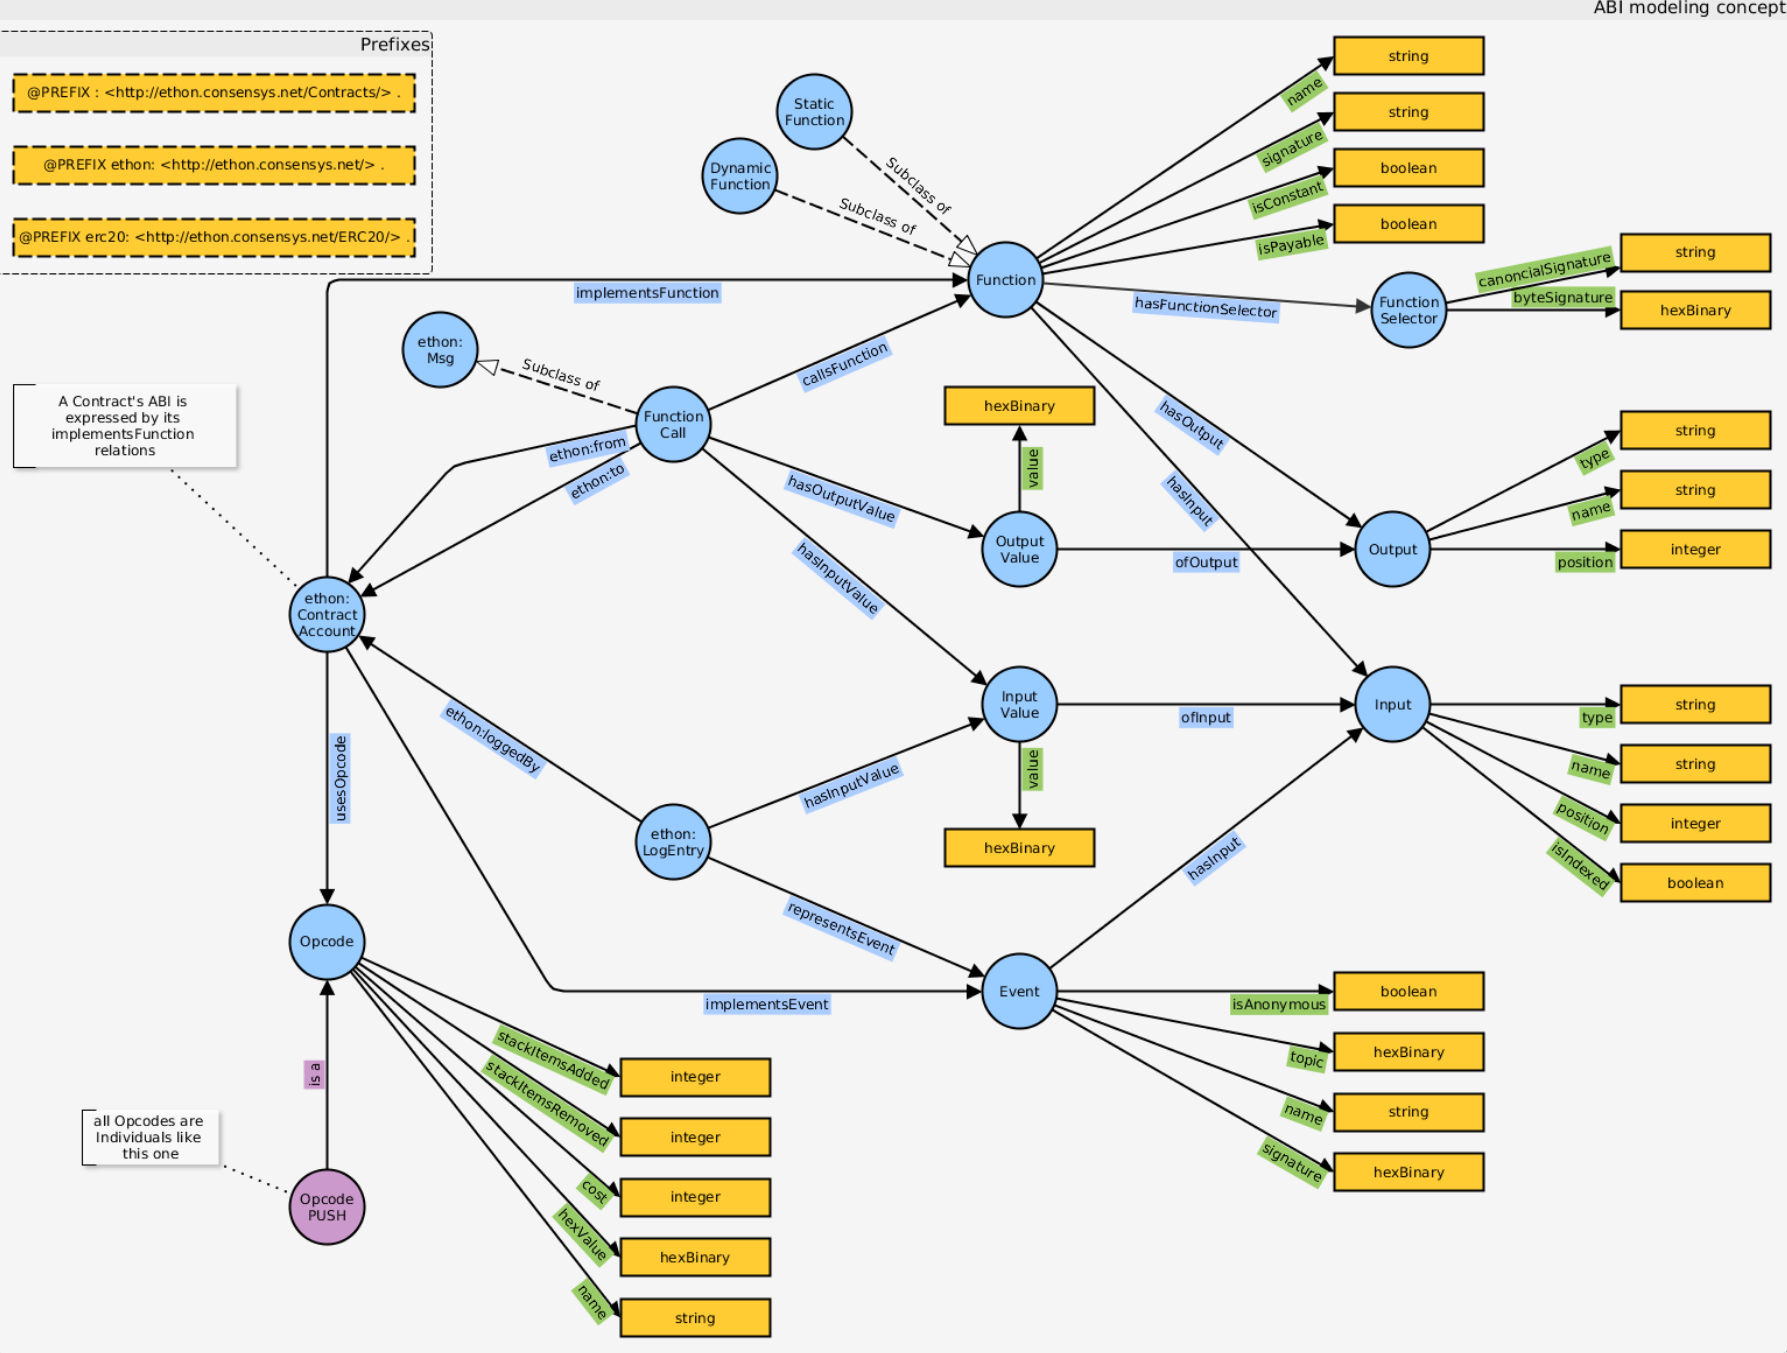
\includegraphics[width=1.80\textwidth]{images/chap2_EthOnContract.png}
		\end{minipage}
		\caption[EthOn classes]{EthOn contract model (the blue arrow is object properties, the green arrow is data properties, the purple circle is an instance and blue one is a class) \cite{Rashid}}
		
	\end{figure}
	
	\begin{figure}[htb!]
		
		\begin{minipage}{0.55\linewidth}
			\centering
			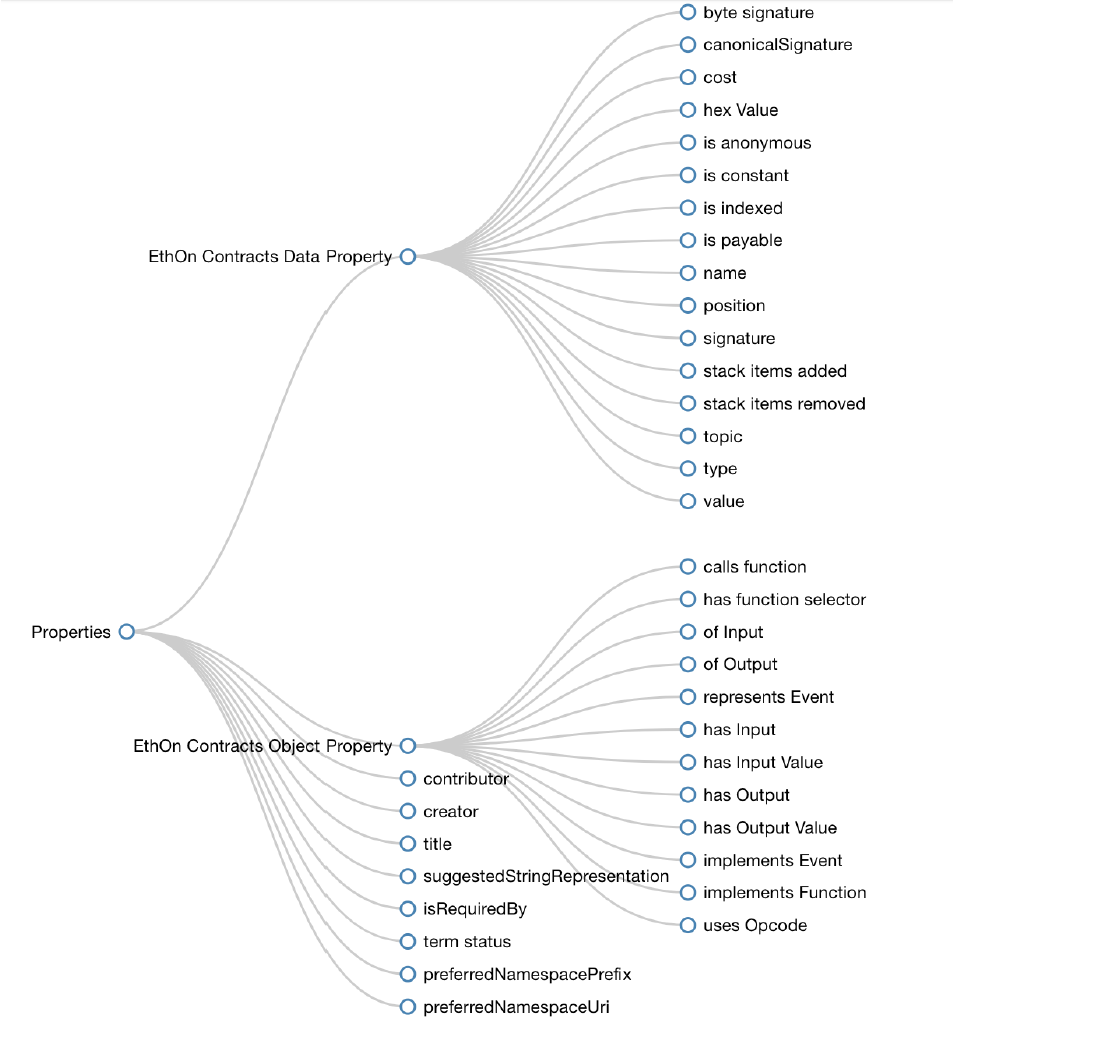
\includegraphics[width=1.65\textwidth]{images/chap02_EthOn_Properties.png}
		\end{minipage}
		\caption[EthOn properties]{EthOn properties \cite{Rashid}}
		
		
	\end{figure}
	
\end{center}
\textbf{\textit{BLONDiE (Blockchain Ontology with Dynamic Extensibility)}} is another OWL ontology that describes the structure of a blockchain similar to EthOn. However, it is less specific than EthOn. Examples include the definitions of terminology like "account," "block," and "transaction" as well as some properties like "transaction payload" or "miner address" in EthOn and BLONDiE. Other terms for various blockchains, such as "BitcoinBlockHeader" and "EthereumBlockHeader," are defined by BLONDiE as subclasses of "BlockHeader." Currently, BLONDiE supports two cryptocurrencies, such as Bitcoin and Ethereum, in which all connections and relationships among objects and characteristics are expressed using the RDF (Resource Description Framework) format \cite{Third}.
\begin{center}
	\begin{figure}[htb!]
		
		\begin{minipage}{0.55\linewidth}
			\centering
			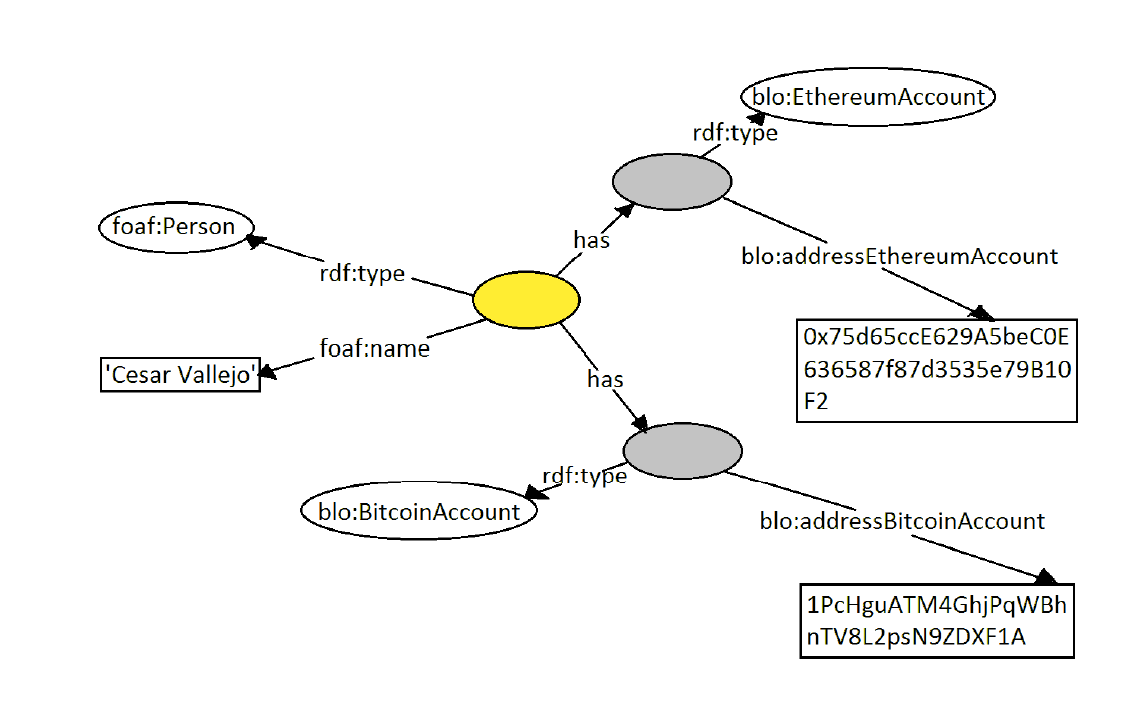
\includegraphics[width=1.75\textwidth]{images/chap02_BLONDiE.png}
		\end{minipage}
		\caption[BLONDiE]{BLONDiE usage example \cite{Hector}}
		
		
	\end{figure}
	
\end{center}
\subsection{Vocabulary in Smart Contract}
As was already noted, two concepts that can be employed for smart contracts are EthOn and BLONDiE. We may be able to annotate smart contracts thanks to several works on HTTP-APIs and semantic annotation of the web. Although the implementation may vary and the contracts are not on web APIs, the fundamental idea remains the same. In other words, smart contracts are annotated using the same vocabulary as are used to annotate web services. Due to their profitability, it appears that distributed ledgers, smart contracts, and web services will frequently be combined \cite{Third}.

\section{Semantify Blockchain}
\subsection{Semantic Blockchain}
Recent growth in the adoption of blockchain technology has increased the demand for semantic reasoning on the distributed ledger as well. To implement semantic web principles in this technology and add a new trusted attribute to a dataset, the blockchain is the best platform. \\
The idea of using semantic web technology with blockchain is new, and how to implement it with smart contracts is also up for debate\\
The following are some \textbf{definitions of semantic  blockchain:} \\
\textit{- Semantic blockchain is the application of semantic web standards on the blockchain; these standards are based on RDF.}\\
\textit{-Semantic blockchain is the representation of stored data on a distributed ledger using linked data \cite{Hector}.}\\
\subsection{Semantification Process}
The industrial world is impacted by semantic blockchain or semantic distributed ledger, and as a result, new applications and frameworks are being developed to bridge the two worlds. \\ 
There are some ways to semantify blockchain, as follows:\\
\textbf{-} Converting blockchain data to RDF while using vocabulary, ontology, and other tools. \\
Due to the high cost of data storage in blockchains, the only viable option is to first save the hash point to the dataset in the blockchain before sharing RDF. \\
Building a semantic blockchain to communicate internal data protocols in RDF \cite{Hector}. 
\subsection{Semantic Ontology Mapping Using BLONDiE}
The basic blockchain elements must be mapped to the pertinent semantic web terms, concepts, and ontologies in order for the system to produce RDF. The BLONDiE query has been enhanced in two ways to improve efficiency: First, an attribute for each entity's hash has been added to records pertaining to blocks and transactions. Second, records pertaining to the transactions have been enhanced with references to other objects, such as blocks or smart contracts. \\
Blockchain only keeps a binary form of each contract together with its associated metadata. The Application Binary Interface (ABI) standard is necessary in order to communicate with the contract. This specification, which is formed when a smart contract is put together and kept on the blockchain, is in the form of JSON. The ABI establishes all contract functions and offers descriptions of each contract's input and output parameters \cite{Third}.
\begin{center}
	\begin{figure}[htb!]
		
		\begin{minipage}{0.45\linewidth}
			\centering
			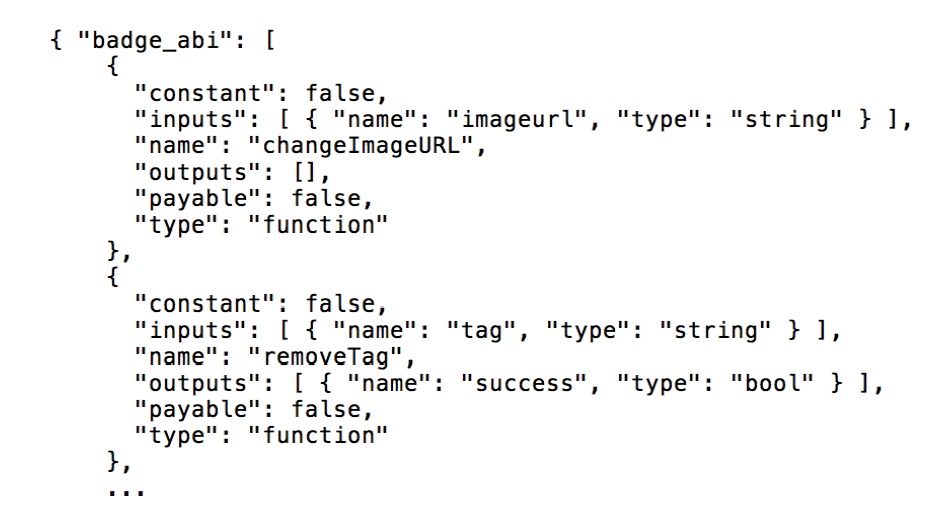
\includegraphics[width=1.95\textwidth]{images/chap02_SmartContract_ABI.png}
		\end{minipage}
		\caption[Smart contract application binary interface (ABI)]{Smart contract application Bbinary interface (ABI)}
		
	\end{figure}
	
\end{center}